% Provenance (never printed): cycle 4 SVT, "La planete Terre": the dynamics of
% the Earth's outer shell, plates and their boundaries, continental drift as a
% history of ideas; see sources/outline_sources.md. Pilot chapter, 2026-10-22.
\chapter{Tectônica de placas: o quebra-cabeça que se move}\label{ch:g7:plate-tectonics}

Abra um \omterm{def:g3:continents-and-oceans:world-map}{mapa-múndi} sobre a mesa e observe as duas margens do \omterm{def:g2:water-on-earth:ocean}{oceano}
Atlântico. A grande saliência do Brasil parece feita para se encaixar no
recôncavo da costa oeste da África, como se alguém tivesse cortado um único
pedaço de terra em dois e afastado as metades. As primeiras pessoas que
imprimiram bons \omterm{def:g2:drawing-to-map:map}{mapas} das duas costas notaram isso na hora. Durante três
séculos, isso continuou sendo uma curiosidade. No século XX, virou o
ponto de partida da teoria que hoje explica por que o chão treme no Japão,
por que os Andes são tão altos, por que a Islândia fica cada vez mais
larga --- e por que o \omterm{def:g2:drawing-to-map:map}{mapa} sobre a mesa é só um retrato instantâneo de um
mundo que se move.

\begin{omfigure}
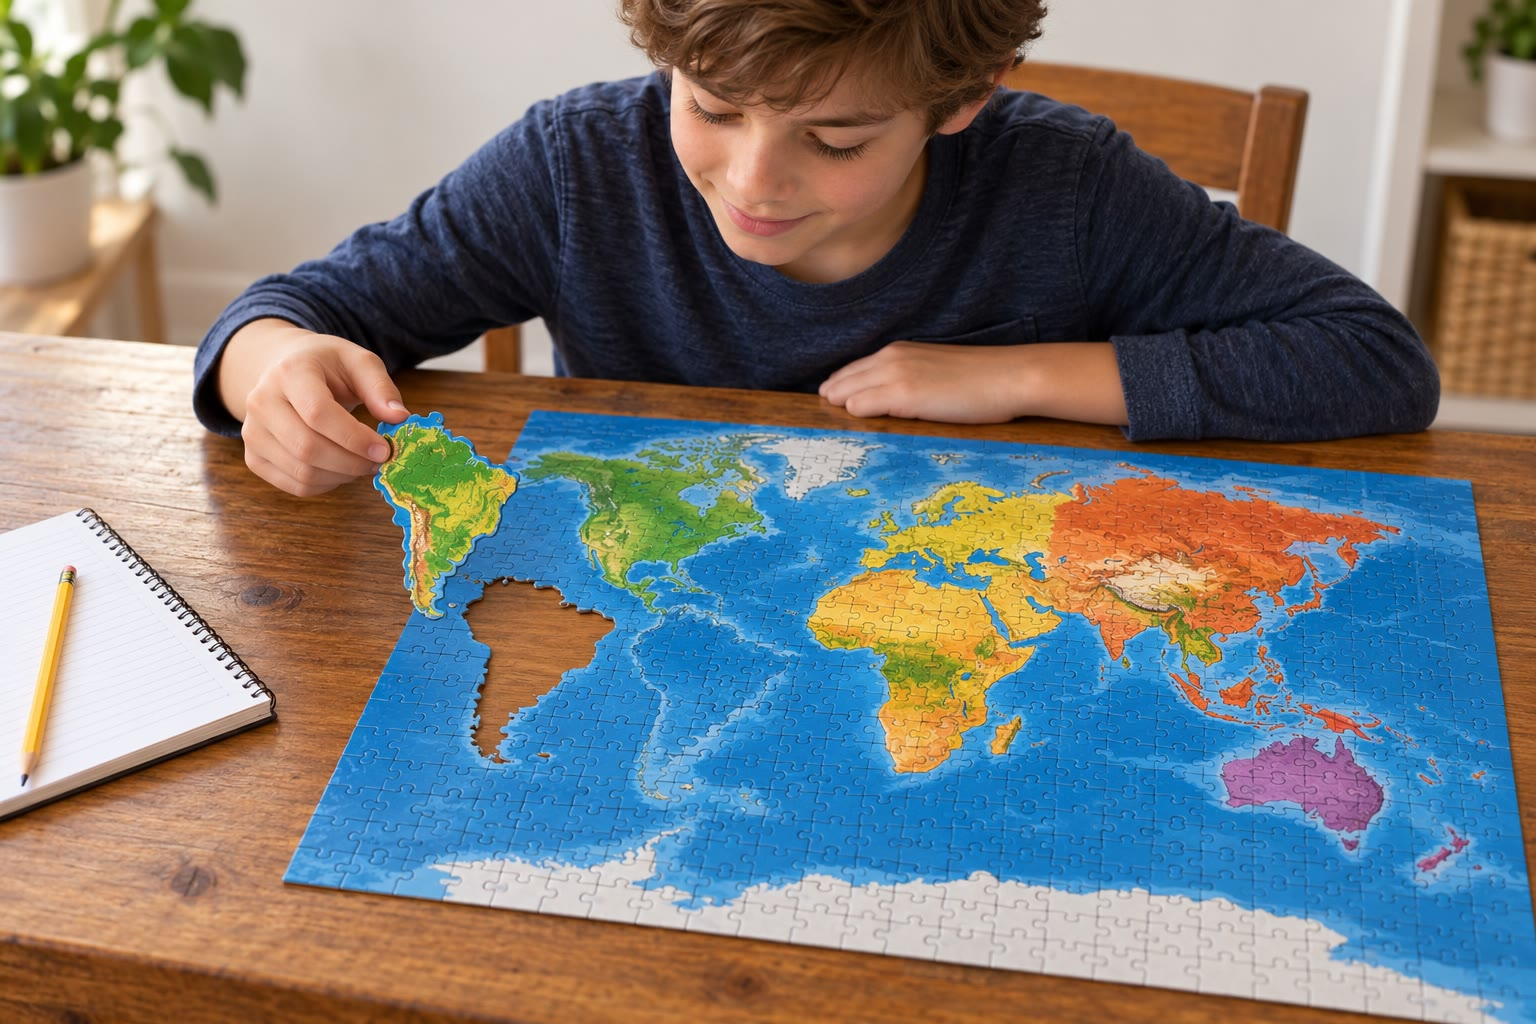
\includegraphics[width=0.62\linewidth]{images/book1/ai/g7-puzzle-map.jpg}

{\small A América do Sul ao lado da África: num quebra-cabeça, o encaixe é
um jogo; na Terra de verdade, é uma pista.}
\end{omfigure}

\begin{recall}
A Terra tem três camadas principais: uma \emph{\omterm{def:g6:inside-the-earth:layers}{crosta}} fina e rochosa, um
\emph{\omterm{def:g6:inside-the-earth:layers}{manto}} grosso de \omterm{def:g3:stones-pebbles-sand:rock}{rocha} quente e um \emph{\omterm{def:g6:inside-the-earth:layers}{núcleo}} metálico; a
temperatura sobe com a profundidade (\cref{ch:g6:inside-the-earth}). Um
lugar no \omterm{def:g3:continents-and-oceans:globe}{globo} é localizado pela sua \omterm{def:g6:latitude-longitude:latitude}{latitude} e pela sua \omterm{def:g6:latitude-longitude:longitude}{longitude}
(\cref{ch:g6:latitude-longitude}).
\end{recall}

\section{Continentes que já se encaixaram}

\begin{definition}[Deriva continental]\label{def:g7:plate-tectonics:continental-drift}
A \emph{deriva continental}\index{deriva continental} é a ideia de que os
\omterm{def:g3:continents-and-oceans:continent}{continentes} se deslocam devagar pela superfície da Terra, de modo que as
suas posições, e as formas dos \omterm{def:g2:water-on-earth:ocean}{oceanos} entre eles, mudaram ao longo das
eras.
\end{definition}

\begin{definition}[Supercontinente]\label{def:g7:plate-tectonics:supercontinent}
Um \emph{supercontinente}\index{supercontinente} é uma única massa de terra
formada por todos, ou quase todos, os \omterm{def:g3:continents-and-oceans:continent}{continentes} juntos. O último, a
\emph{Pangeia}\index{Pangeia} (``todas as terras'', em grego), começou a se
partir entre cerca de 225 e 200 milhões de anos atrás.
% ledger: usgs:pangaea-breakup
\end{definition}

O cientista que defendeu a \omterm{def:g7:plate-tectonics:continental-drift}{deriva continental} como uma teoria de verdade,
com provas, foi Alfred Wegener. Ele reuniu quatro tipos de pistas.

\begin{enumerate}
  \item \textbf{As formas das costas.} A América do Sul e a África se
        encaixam como duas peças de um quebra-cabeça, e o mesmo acontece
        com vários outros \omterm{def:g1:landscapes-around-us:water}{litorais}.
  \item \textbf{Os fósseis.} Os mesmos animais e plantas fósseis são
        encontrados em \omterm{def:g3:continents-and-oceans:continent}{continentes} que hoje estão separados por milhares de
        quilômetros de \omterm{def:g2:water-on-earth:ocean}{oceano}. O \emph{Mesosaurus} era um pequeno réptil que
        vivia em \omterm{def:g2:water-on-earth:salt-fresh}{água doce}: ele não poderia ter atravessado um \omterm{def:g2:water-on-earth:ocean}{oceano} a
        nado, e mesmo assim os seus fósseis estão tanto no Brasil quanto no
        sul da África.
  \item \textbf{As \omterm{def:g3:stones-pebbles-sand:rock}{rochas}.} \omterm{def:g3:stones-pebbles-sand:rock}{Rochas} dos mesmos tipos e das mesmas idades, e
        antigas cadeias de \omterm{def:g1:landscapes-around-us:landform}{montanhas} da mesma forma, param numa costa e
        recomeçam na costa oposta, como as linhas de um jornal rasgado.
  \item \textbf{Os \omterm{def:g5:weather-and-climate:climate}{climas} antigos.} O carvão, formado a partir das plantas
        de florestas quentes e pantanosas, é encontrado na Antártida; marcas
        deixadas por antigas geleiras são encontradas em partes da África
        que hoje são quentes e áridas. Essas terras devem ter ficado, um dia,
        em outros \omterm{def:g5:weather-and-climate:climate}{climas}, em outras \omterm{def:g6:latitude-longitude:latitude}{latitudes}.
\end{enumerate}
% ledger: usgs:coal-antarctica, usgs:fossil-map

\begin{omfigure}
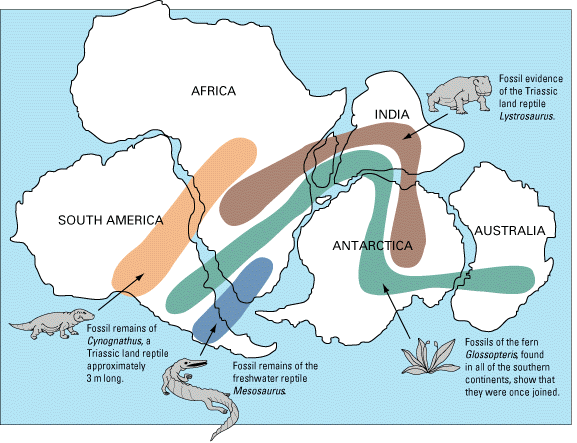
\includegraphics[width=0.86\linewidth]{images/book1/g7-usgs-fossil-map.png}

{\small Os \omterm{def:g3:continents-and-oceans:continent}{continentes} do sul encaixados de novo. Cada faixa colorida liga
os lugares onde hoje se encontra uma espécie fóssil: os répteis terrestres
\emph{Cynognathus} e \emph{Lystrosaurus}, o réptil de \omterm{def:g2:water-on-earth:salt-fresh}{água doce}
\emph{Mesosaurus} e a samambaia \emph{Glossopteris}. Separados, os
\omterm{def:g3:continents-and-oceans:continent}{continentes} espalham as faixas; juntos, as faixas continuam sem
interrupção. \omterm{def:g2:drawing-to-map:map}{Mapa}: U.S. Geological Survey, \emph{This Dynamic Earth}
(domínio público).}
\end{omfigure}

\begin{history}[A ideia de Wegener, 1912--1930]
% ledger: usgs:wegener-1912, usgs:wegener-death, usgs:jeffreys
Alfred Wegener, um meteorologista alemão de 32 anos, apresentou a teoria da
\omterm{def:g7:plate-tectonics:continental-drift}{deriva continental} em dois artigos em 1912. A maioria dos geólogos a
rejeitou. A objeção mais forte era que Wegener não conseguia dizer
\emph{o que} movia os \omterm{def:g3:continents-and-oceans:continent}{continentes}: ele achava que eles abriam caminho
através da \omterm{def:g3:stones-pebbles-sand:rock}{rocha} do fundo do \omterm{def:g2:water-on-earth:ocean}{oceano}, e o físico Harold Jeffreys mostrou que
\omterm{def:g3:continents-and-oceans:continent}{continentes} sólidos não conseguiriam fazer isso sem se despedaçar. Wegener
continuou reunindo provas até morrer na calota de gelo da Groenlândia, em
1930, durante uma expedição. A resposta que lhe faltava veio do fundo dos
\omterm{def:g2:water-on-earth:ocean}{oceanos}, explorado depois dos anos 1950: ela é contada num ano mais
adiante.
\end{history}

\section{As placas}

As pistas de Wegener estavam certas, mas os seus \omterm{def:g3:continents-and-oceans:continent}{continentes} eram as peças
erradas. Não são só os \omterm{def:g3:continents-and-oceans:continent}{continentes} que se movem: toda a casca externa da
Terra, tanto embaixo dos \omterm{def:g3:continents-and-oceans:continent}{continentes} quanto embaixo dos \omterm{def:g2:water-on-earth:ocean}{oceanos}, está
partida em pedaços.

\begin{definition}[Placa tectônica]\label{def:g7:plate-tectonics:plate}
Uma \emph{placa tectônica}\index{placa tectonica@placa tectônica} (ou simplesmente uma
placa) é uma grande laje rígida de \omterm{def:g3:stones-pebbles-sand:rock}{rocha} que forma parte da casca externa
da Terra. Uma placa é feita da \omterm{def:g6:inside-the-earth:layers}{crosta} e da parte mais alta, fria e rígida
do \omterm{def:g6:inside-the-earth:layers}{manto}, que juntas têm pelo menos 80 quilômetros de espessura em média;
ela se desloca devagar sobre o \omterm{def:g6:inside-the-earth:layers}{manto} mais quente e mais mole que fica
embaixo dela.
% ledger: usgs:lithosphere-80km
\end{definition}

\begin{definition}[Tectônica de placas]\label{def:g7:plate-tectonics:plate-tectonics}
A \emph{tectônica de placas}\index{tectonica de placas@tectônica de placas} é a teoria segundo a
qual a casca externa da Terra está dividida em placas que se movem umas em
relação às outras, e a maioria dos \omterm{def:g4:volcanoes-earthquakes-first-look:earthquake}{terremotos}, dos \omterm{def:g4:volcanoes-earthquakes-first-look:volcano}{vulcões} e das
\omterm{def:g4:world-physical-map:range}{cordilheiras} se forma onde as \omterm{def:g7:plate-tectonics:plate}{placas} se encontram.
\end{definition}

\begin{remark}[Quantas placas?]\label{rem:g7:plate-tectonics:how-many}
% ledger: usgs:plates-dozen, pb2002:count
Cerca de uma dúzia de \omterm{def:g7:plate-tectonics:plate}{placas} são grandes; muitas outras são pequenas. Um
\omterm{def:g2:drawing-to-map:map}{mapa} detalhado usado pelos geólogos conta 52 delas. Uma \omterm{def:g7:plate-tectonics:plate}{placa} pode levar um
\omterm{def:g3:continents-and-oceans:continent}{continente}, um \omterm{def:g2:water-on-earth:ocean}{oceano} ou os dois: a \omterm{def:g7:plate-tectonics:plate}{placa} Sul-Americana leva toda a
América do Sul e a metade oeste do Atlântico Sul. A \omterm{def:g7:plate-tectonics:plate}{placa} do Pacífico, a
maior, quase não leva terra nenhuma.
\end{remark}

\begin{omfigure}
\begin{tikzpicture}
\begin{axis}[ommap, width=\linewidth, xtick={-180,-90,...,180}, ytick={-60,0,60}]
\addplot[fill=omLithAlluv, draw=black!45, line width=0.2pt] table {figdata/out/shared-geo-land.dat};
\addplot[omRidge, line width=0.8pt] table {figdata/out/shared-geo-school-ridge.dat};
\addplot[omRidge!70!black, line width=0.8pt] table {figdata/out/shared-geo-school-transform.dat};
\addplot[omTrench, line width=0.8pt] table {figdata/out/shared-geo-school-subduction.dat};
\addplot[fill=omTrench, draw=none] table {figdata/out/shared-geo-school-teeth.dat};
\addplot[black!65, line width=0.8pt] table {figdata/out/shared-geo-school-collision.dat};
\begin{scope}[every node/.style={font=\scriptsize\bfseries, text=black!85,
    fill=white, fill opacity=0.75, text opacity=1, inner sep=1pt, align=center}]
  \node at (axis cs:-150,12) {Pacífica};
  \node at (axis cs:-103,52) {Norte-\\-Americana};
  \node at (axis cs:-48,-12) {Sul-\\-Americana};
  \node at (axis cs:85,57) {Euro-Asiática};
  \node at (axis cs:18,8) {Africana};
  \node at (axis cs:10,-75) {Antártica};
  \node at (axis cs:78,11) {Indiana};
  \node at (axis cs:128,-26) {Australiana};
  \node at (axis cs:-95,-22) {de Nazca};
  \node at (axis cs:50,20) {Arábica};
\end{scope}
\end{axis}
\end{tikzpicture}

{\small As principais \omterm{def:g7:plate-tectonics:plate}{placas tectônicas}. Em vermelho: \omterm{def:g7:plate-tectonics:plate}{placas} que se
afastam; em azul com triângulos: uma \omterm{def:g7:plate-tectonics:plate}{placa} que afunda embaixo da outra (os
triângulos ficam na \omterm{def:g7:plate-tectonics:plate}{placa} que continua em cima); em cinza: \omterm{def:g7:plate-tectonics:plate}{placas} que se
empurram ao longo de uma larga zona de \omterm{def:g1:landscapes-around-us:landform}{montanhas}; em vermelho-escuro:
\omterm{def:g7:plate-tectonics:plate}{placas} que deslizam uma ao lado da outra. Limites segundo P.~Bird (2003);
litorais de Natural Earth.}
\end{omfigure}

Como sabemos onde uma \omterm{def:g7:plate-tectonics:plate}{placa} termina e a seguinte começa? Observe onde a
Terra é agitada.

\begin{proposition}[Os terremotos e os vulcões traçam os limites das placas]\label{prop:g7:plate-tectonics:restless}
% ledger: data:usgs-comcat, data:pb2002 (share computed in figdata/grade-7/quakes_on_boundaries.py)
Os \omterm{def:g4:volcanoes-earthquakes-first-look:earthquake}{terremotos} e os \omterm{def:g4:volcanoes-earthquakes-first-look:volcano}{vulcões} não estão espalhados ao acaso pela Terra: a
maioria deles fica ao longo de faixas estreitas, e essas faixas são as
bordas das \omterm{def:g7:plate-tectonics:plate}{placas}. Dos 7\,031 \omterm{def:g4:volcanoes-earthquakes-first-look:earthquake}{terremotos} de magnitude 6 ou mais
registrados entre 1976 e 2025, 6\,472 --- ou seja, 92\,\% --- aconteceram a
menos de \qty{300}{km} de um \omterm{def:g7:plate-tectonics:plate-boundary}{limite de placas}.
\end{proposition}

\begin{omfigure}
\begin{tikzpicture}
\begin{axis}[ommap, width=\linewidth, xtick={-180,-90,...,180}, ytick={-60,0,60},
  legend style={at={(0.02,0.04)}, anchor=south west, font=\scriptsize,
  fill=white, fill opacity=0.85, text opacity=1, draw=black!40}]
\addplot[fill=omLithAlluv, draw=black!45, line width=0.2pt, forget plot] table {figdata/out/shared-geo-land.dat};
\addplot[only marks, mark=*, mark size=0.45pt, omThm!85!black] table[x=lon, y=lat] {figdata/out/grade-7-quakes_on_boundaries-map.dat};
\addlegendentry{terremoto de magnitude 6.5 ou mais, 1976--2025}
\addplot[only marks, mark=triangle*, mark size=1.1pt, black] table {figdata/out/shared-geo-volcanoes.dat};
\addlegendentry{vulcão ativo nos últimos 12\,000 anos}
\end{axis}
\end{tikzpicture}

{\small Os grandes \omterm{def:g4:volcanoes-earthquakes-first-look:earthquake}{terremotos} e os \omterm{def:g4:volcanoes-earthquakes-first-look:volcano}{vulcões} recentes. Compare com o \omterm{def:g2:drawing-to-map:map}{mapa} das
\omterm{def:g7:plate-tectonics:plate}{placas} acima: os pontos e os triângulos desenham os limites das \omterm{def:g7:plate-tectonics:plate}{placas}.
Dados: catálogo de \omterm{def:g4:volcanoes-earthquakes-first-look:earthquake}{terremotos} do U.S. Geological Survey; Smithsonian Global
Volcanism Program.}
\end{omfigure}

\section{Três tipos de limites de placas}

\begin{definition}[Limite de placas]\label{def:g7:plate-tectonics:plate-boundary}
Um \emph{limite de placas}\index{limite de placas} é a linha, ou a zona
estreita, onde duas \omterm{def:g7:plate-tectonics:plate}{placas} se encontram. Conforme o modo como as duas
\omterm{def:g7:plate-tectonics:plate}{placas} se movem uma em relação à outra, um limite é de um destes três
tipos:
\begin{itemize}
  \item num \emph{limite divergente}\index{limite divergente} as duas
        \omterm{def:g7:plate-tectonics:plate}{placas} se afastam;
  \item num \emph{limite convergente}\index{limite convergente} as duas
        \omterm{def:g7:plate-tectonics:plate}{placas} se aproximam;
  \item num \emph{limite transformante}\index{limite transformante} as duas
        \omterm{def:g7:plate-tectonics:plate}{placas} deslizam uma ao lado da outra.
\end{itemize}
\end{definition}

\begin{example}[Limites divergentes: a Islândia e a África Oriental]\label{ex:g7:plate-tectonics:divergent}
% ledger: usgs:iceland, usgs:east-africa
Pelo meio do \omterm{def:g2:water-on-earth:ocean}{oceano} Atlântico corre uma cadeia de \omterm{def:g1:landscapes-around-us:landform}{montanhas} submarinas, a
dorsal mesoatlântica, onde as \omterm{def:g7:plate-tectonics:plate}{placas} dos dois lados se afastam. A \omterm{def:g3:stones-pebbles-sand:rock}{rocha}
quente do \omterm{def:g6:inside-the-earth:layers}{manto} sobe para o espaço aberto, derrete em parte e vira um novo
fundo oceânico: um \omterm{def:g7:plate-tectonics:plate-boundary}{limite divergente} constrói \omterm{def:g7:plate-tectonics:plate}{placa} nova. A Islândia é um
pedaço dessa dorsal que sai acima do \omterm{def:g2:water-on-earth:ocean}{mar}: ali, a América do Norte se
desloca para o oeste e a Eurásia para o leste, e a ilha vai sendo rasgada
devagar. Entre 1975 e 1984, as fendas perto do \omterm{def:g4:volcanoes-earthquakes-first-look:volcano}{vulcão} Krafla, no norte da
ilha, se alargaram cerca de 7 metros no total. Um \omterm{def:g7:plate-tectonics:plate-boundary}{limite divergente} também
pode cortar um \omterm{def:g3:continents-and-oceans:continent}{continente}: ao longo do Rifte da África Oriental, a África
começa a se partir, e o \omterm{def:g2:water-on-earth:ocean}{mar} Vermelho é um \omterm{def:g2:water-on-earth:ocean}{oceano} jovem que já separou a
Arábia da África.
\end{example}

\begin{example}[Limites convergentes: os Andes e o Himalaia]\label{ex:g7:plate-tectonics:convergent}
% ledger: usgs:trench-depth, usgs:himalaya
Na costa oeste da América do Sul, a \omterm{def:g7:plate-tectonics:plate}{placa} de Nazca, que leva \omterm{def:g2:water-on-earth:ocean}{oceano}, se
aproxima da \omterm{def:g7:plate-tectonics:plate}{placa} Sul-Americana, que leva um \omterm{def:g3:continents-and-oceans:continent}{continente}. A \omterm{def:g7:plate-tectonics:plate}{placa} oceânica,
mais pesada, se curva e afunda embaixo do \omterm{def:g3:continents-and-oceans:continent}{continente}, para dentro do
\omterm{def:g6:inside-the-earth:layers}{manto}. Ao longo da linha onde ela desce, o fundo do \omterm{def:g2:water-on-earth:ocean}{mar} mergulha numa fossa
profunda; acima da \omterm{def:g7:plate-tectonics:plate}{placa} que afunda, a terra é sacudida por \omterm{def:g4:volcanoes-earthquakes-first-look:earthquake}{terremotos} e
cheia de \omterm{def:g4:volcanoes-earthquakes-first-look:volcano}{vulcões}: os Andes. No oeste do Pacífico, onde uma \omterm{def:g7:plate-tectonics:plate}{placa} oceânica
afunda embaixo de outra, as fossas são os lugares mais fundos da Terra: a
fossa das Marianas tem quase \qty{11000}{m} de profundidade. Quando dois
\omterm{def:g3:continents-and-oceans:continent}{continentes} se encontram, nenhum dos dois afunda: a \omterm{def:g6:inside-the-earth:layers}{crosta} se amassa e
fica mais grossa. A Índia colidiu com a Ásia há cerca de 50 milhões de
anos, e as duas \omterm{def:g7:plate-tectonics:plate}{placas} ainda se empurram; foi assim que o Himalaia e o
planalto do Tibete se ergueram.
\end{example}

\begin{example}[Um limite transformante: a falha de San Andreas]\label{ex:g7:plate-tectonics:transform}
% ledger: usgs:san-andreas, usgs:san-andreas-photo
Na Califórnia, a \omterm{def:g7:plate-tectonics:plate}{placa} do Pacífico desliza para o noroeste ao lado da \omterm{def:g7:plate-tectonics:plate}{placa}
Norte-Americana, ao longo da falha de San Andreas, com cerca de
\qty{1300}{km} de comprimento. Nenhuma \omterm{def:g7:plate-tectonics:plate}{placa} é criada ou destruída ali; as
duas \omterm{def:g7:plate-tectonics:plate}{placas} se raspam, e os trancos dessa raspagem são \omterm{def:g4:volcanoes-earthquakes-first-look:earthquake}{terremotos}.
\end{example}

\begin{omfigure}
\begin{tikzpicture}[x=1cm, y=1cm, font=\small]
  % mantle
  \fill[omLithGranite!45] (0,-3.3) rectangle (12.4,-0.85);
  \node[font=\footnotesize, text=black!75] at (2.6,-2.6) {manto: quente e mole};
  % sea water
  \fill[omSea] (0,0) -- (0,-0.75) -- (1.5,-0.6) -- (3,-0.25) -- (4.5,-0.6)
    -- (7.4,-0.8) -- (8.0,-1.2) -- (8.6,-0.6) -- (8.9,0) -- cycle;
  % oceanic plates (the ridge at x = 3, the trench at x = 8)
  \fill[omLithBasalt!70] (0,-0.75) -- (1.5,-0.6) -- (3,-0.25) -- (4.5,-0.6)
    -- (7.4,-0.8) -- (8.0,-1.2) -- (9.6,-2.3) -- (10.2,-3.3) -- (9.5,-3.3)
    -- (8.6,-2.2) -- (7.5,-1.55) -- (4.5,-1.35) -- (3.2,-0.95) -- (2.8,-0.95)
    -- (1.5,-1.35) -- (0,-1.45) -- cycle;
  % continental plate
  \fill[omLithSand!80] (8.6,-0.6) -- (8.9,0) -- (9.4,0.35) -- (9.8,0.9)
    -- (10.2,0.35) -- (12.4,0.2) -- (12.4,-1.9) -- (10.6,-1.9) -- (9.6,-2.3)
    -- (8.0,-1.2) -- cycle;
  \draw[black!70, line width=0.5pt] (0,-0.75) -- (1.5,-0.6) -- (3,-0.25)
    -- (4.5,-0.6) -- (7.4,-0.8) -- (8.0,-1.2) -- (8.6,-0.6) -- (8.9,0)
    -- (9.4,0.35) -- (9.8,0.9) -- (10.2,0.35) -- (12.4,0.2);
  \draw[black!45, densely dashed] (0,0) -- (8.9,0);
  % magma: under the ridge and under the volcano
  \fill[omThm!80] (2.85,-0.95) -- (3,-0.3) -- (3.15,-0.95) -- cycle;
  \draw[omThm!80, line width=1.4pt, -{Stealth[length=2.2mm]}] (3,-1.85) -- (3,-1.0);
  \draw[omThm!80, line width=1.2pt, decorate, decoration={snake, amplitude=0.6pt,
    segment length=4pt}] (9.8,-2.45) -- (9.8,0.75);
  % plate motions
  \draw[black, line width=1pt, -{Stealth[length=2.4mm]}] (2.5,-0.75) -- (1.3,-0.95);
  \draw[black, line width=1pt, -{Stealth[length=2.4mm]}] (3.5,-0.75) -- (5.4,-1.05);
  \draw[black, line width=1pt, -{Stealth[length=2.4mm]}] (12.1,-0.85) -- (10.9,-0.85);
  \draw[black, line width=1pt, -{Stealth[length=2.4mm]}] (8.7,-1.75) -- (9.3,-2.25);
  % labels
  \node[font=\footnotesize, align=center, above] at (3,0.05) {limite divergente:\\dorsal oceânica};
  \node[font=\footnotesize, align=center, below] at (6.9,-1.95) {limite convergente:\\a placa oceânica afunda};
  \draw[black!60, thin] (8.0,-1.25) -- (7.6,-1.9);
  \node[font=\footnotesize, above] at (8.0,0.05) {fossa};
  \draw[black!60, thin] (8.0,0.05) -- (8.0,-1.1);
  \node[font=\footnotesize, above] at (9.8,0.95) {vulcão};
  \node[font=\footnotesize] at (11.4,-0.4) {continente};
  \node[font=\footnotesize] at (1.2,-1.6) {placa oceânica};
  \node[font=\footnotesize, text=black!70] at (5.6,-0.32) {oceano};
\end{tikzpicture}

\medskip
\begin{tikzpicture}[font=\small]
  \fill[omLithBasalt!45] (0,0) rectangle (2.4,2.2);
  \fill[omLithSand!70] (2.4,0) rectangle (4.8,2.2);
  \draw[fault] (2.4,-0.1) -- (2.4,2.3);
  \draw[black, line width=1pt, -{Stealth[length=2.4mm]}] (1.2,0.5) -- (1.2,1.7);
  \draw[black, line width=1pt, -{Stealth[length=2.4mm]}] (3.6,1.7) -- (3.6,0.5);
  \node[font=\footnotesize, below] at (1.2,-0.1) {placa A};
  \node[font=\footnotesize, below] at (3.6,-0.1) {placa B};
  \node[font=\footnotesize, align=left, anchor=west] at (5.1,1.1)
    {limite transformante, visto de cima:\\as placas deslizam uma ao lado da outra;\\nenhuma placa é criada ou destruída};
\end{tikzpicture}

{\small Em cima: um corte através de dois \omterm{def:g7:plate-tectonics:plate-boundary}{limites de placas} (fora de
escala; as profundidades estão muito exageradas). Na dorsal, as \omterm{def:g7:plate-tectonics:plate}{placas} se
afastam e a \omterm{def:g3:stones-pebbles-sand:rock}{rocha} quente sobe do \omterm{def:g6:inside-the-earth:layers}{manto}; na fossa, a \omterm{def:g7:plate-tectonics:plate}{placa} oceânica afunda
embaixo do \omterm{def:g3:continents-and-oceans:continent}{continente}, e a \omterm{def:g3:stones-pebbles-sand:rock}{rocha} que derrete acima dela alimenta \omterm{def:g4:volcanoes-earthquakes-first-look:volcano}{vulcões}.
Embaixo: um \omterm{def:g7:plate-tectonics:plate-boundary}{limite transformante} visto de cima.}
\end{omfigure}

\begin{omfigure}
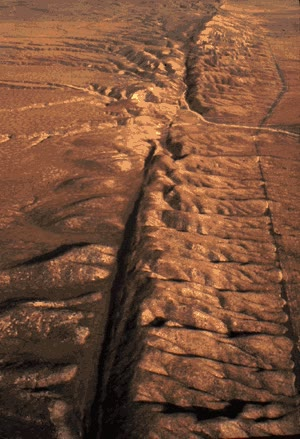
\includegraphics[width=0.28\linewidth]{images/book1/g7-usgs-san-andreas.jpg}

{\small A falha de San Andreas atravessando a \omterm{def:g1:landscapes-around-us:landform}{planície} de Carrizo, na
Califórnia, vista de um avião: o longo \omterm{def:g1:landscapes-around-us:landform}{vale} reto é o limite entre a \omterm{def:g7:plate-tectonics:plate}{placa}
do Pacífico (à esquerda) e a \omterm{def:g7:plate-tectonics:plate}{placa} Norte-Americana (à direita). Foto:
Robert E. Wallace, U.S. Geological Survey (domínio público).}
\end{omfigure}

\begin{method}[Reconhecer um limite de placas num mapa]\label{met:g7:plate-tectonics:recognise}
Para decidir que tipo de limite separa duas \omterm{def:g7:plate-tectonics:plate}{placas}:
\begin{enumerate}
  \item encontre, num \omterm{def:g2:drawing-to-map:map}{mapa} dos movimentos das \omterm{def:g7:plate-tectonics:plate}{placas}, as setas dos dois
        lados do limite;
  \item se elas apontam para longe do limite, ele é divergente; se apontam
        para ele, convergente; se são paralelas a ele e apontam em sentidos
        opostos, transformante;
  \item confira com a \omterm{def:g1:landscapes-around-us:landscape}{paisagem}: uma dorsal no meio de um \omterm{def:g2:water-on-earth:ocean}{oceano} ou um rifte
        atravessando um \omterm{def:g3:continents-and-oceans:continent}{continente} acompanham um \omterm{def:g7:plate-tectonics:plate-boundary}{limite divergente}; uma
        fossa profunda com uma fileira de \omterm{def:g4:volcanoes-earthquakes-first-look:volcano}{vulcões}, ou uma \omterm{def:g4:world-physical-map:range}{cordilheira} alta,
        um \omterm{def:g7:plate-tectonics:plate-boundary}{limite convergente}; uma longa falha reta sem nenhum dos dois, um
        \omterm{def:g7:plate-tectonics:plate-boundary}{limite transformante}.
\end{enumerate}
\end{method}

\section{Com que velocidade as placas se movem?}

\begin{proposition}[Alguns centímetros por ano]\label{prop:g7:plate-tectonics:speed}
% ledger: data:pb2002 (speeds computed in figdata/grade-7/plate_speeds.py), usgs:mar-rate
Duas \omterm{def:g7:plate-tectonics:plate}{placas} vizinhas se movem uma em relação à outra a uma velocidade de
alguns centímetros por ano: de cerca de 2 centímetros por ano no Atlântico
Norte a mais de 14 centímetros por ano na dorsal do Pacífico Leste, a
dorsal que se abre mais depressa na Terra.
\end{proposition}

\begin{omfigure}
\begin{tikzpicture}
\begin{axis}[xbar, width=0.82\linewidth, height=5.4cm, xmin=0, xmax=16.5,
  ytick={1,...,6}, yticklabels={dorsal do Atlântico Norte, dorsal do Atlântico Sul,
  falha de San Andreas, Himalaia, fossa Peru--Chile, dorsal do Pacífico Leste},
  y tick label style={font=\small}, tick label style={font=\small},
  xlabel={velocidade de uma placa em relação à outra (cm por ano)},
  label style={font=\small}, bar width=7pt, axis x line=bottom,
  axis y line=left, axis line style={-}, enlarge y limits=0.12,
  nodes near coords, nodes near coords style={font=\scriptsize},
  every node near coord/.append style={/pgf/number format/fixed,
  /pgf/number format/precision=1, /pgf/number format/fixed zerofill}]
\addplot[fill=omDef!55, draw=omDef!80!black] table[x=speed_cm_a, y=rank] {figdata/out/grade-7-plate_speeds.dat};
\end{axis}
\end{tikzpicture}

{\small A velocidade das \omterm{def:g7:plate-tectonics:plate}{placas} em seis limites: médias ao longo de cada
limite calculadas a partir do modelo de \omterm{def:g7:plate-tectonics:plate}{placas} de P.~Bird (2003).}
\end{omfigure}

\begin{method}[De centímetros por ano para quilômetros por milhão de anos]\label{met:g7:plate-tectonics:convert}
Um quilômetro tem \num{100000} centímetros. Uma velocidade de \qty{1}{cm}
por ano, mantida durante um milhão de anos, percorre então \num{1000000}
centímetros, ou seja, \qty{10}{km}. Portanto:
\[
  1\ \text{cm por ano} = 10\ \text{km por milhão de anos}.
\]
Multiplique uma velocidade em centímetros por ano por 10 para obter
quilômetros por milhão de anos; depois multiplique por um número de milhões
de anos para obter uma distância em quilômetros, ou divida uma distância
pela velocidade para obter um tempo.
\end{method}

\begin{example}[O Atlântico cresce]\label{ex:g7:plate-tectonics:atlantic}
% ledger: usgs:mar-rate
Em média, os dois lados da dorsal mesoatlântica se afastam cerca de
\qty{2.5}{cm} por ano, ou seja, \qty{25}{km} por milhão de anos. Em 100
milhões de anos, isso dá \qty{2500}{km}: mantida por tempo suficiente, uma
velocidade lenta demais para ser notada numa vida inteira abre um \omterm{def:g2:water-on-earth:ocean}{oceano}.
\end{example}

\begin{remark}[Medir o movimento hoje]\label{rem:g7:plate-tectonics:gps}
% ledger: usgs:gps
Movimentos tão lentos agora são medidos diretamente. Estações permanentes
presas ao \omterm{def:g3:stones-pebbles-sand:rock}{substrato rochoso} recebem os sinais dos satélites de
posicionamento e calculam a sua própria posição, dia após dia, com
precisão de alguns milímetros. Em alguns anos, vemos estações em placas
diferentes se afastarem ou se aproximarem, às velocidades encontradas
pelas \omterm{def:g3:stones-pebbles-sand:rock}{rochas} ao longo de milhões de anos. O próprio posicionamento por
satélite é o assunto do \cref{ch:g9:maps-of-the-earth}.
\end{remark}

\begin{omfigure}
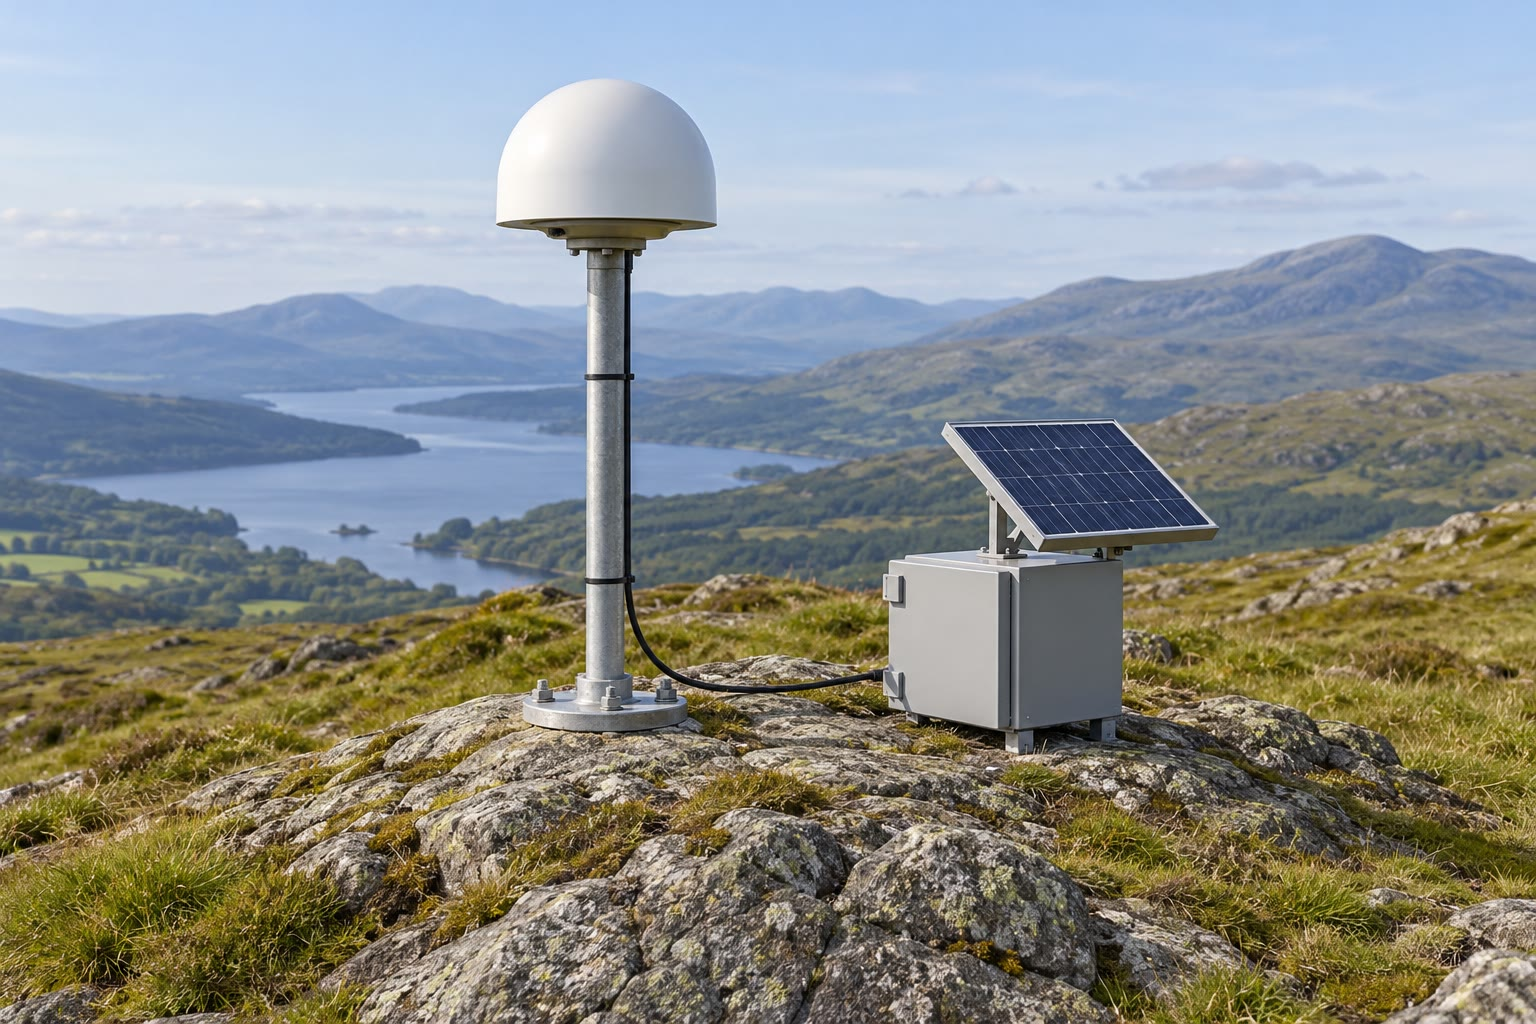
\includegraphics[width=0.55\linewidth]{images/book1/ai/g7-gps-station.jpg}

{\small Uma estação permanente de posicionamento: a sua antena está
aparafusada na \omterm{def:g3:stones-pebbles-sand:rock}{rocha}, então ela se move com a \omterm{def:g7:plate-tectonics:plate}{placa}.}
\end{omfigure}

\section{Exercícios}

\begin{exercise}[$\star$]\label{exo:g7:plate-tectonics:1}
O que é a \omterm{def:g7:plate-tectonics:continental-drift}{deriva continental}? Dê os quatro tipos de pistas que Wegener usou
para defendê-la.
\end{exercise}

\begin{exercise}[$\star$]\label{exo:g7:plate-tectonics:2}
Dê o nome dos três tipos de \omterm{def:g7:plate-tectonics:plate-boundary}{limite de placas} e diga, para cada um, como as
duas \omterm{def:g7:plate-tectonics:plate}{placas} se movem uma em relação à outra.
\end{exercise}

\begin{exercise}[$\star$]\label{exo:g7:plate-tectonics:3}
Observe o \omterm{def:g2:drawing-to-map:map}{mapa} dos \omterm{def:g4:volcanoes-earthquakes-first-look:earthquake}{terremotos} e dos \omterm{def:g4:volcanoes-earthquakes-first-look:volcano}{vulcões}. Dê o nome de duas regiões do
mundo com muitos grandes \omterm{def:g4:volcanoes-earthquakes-first-look:earthquake}{terremotos}, e de um \omterm{def:g3:continents-and-oceans:continent}{continente} que quase não tem
nenhum no seu interior.
\end{exercise}

\begin{exercise}[$\star$]\label{exo:g7:plate-tectonics:4}
Fósseis de \emph{Mesosaurus}, um pequeno réptil que vivia em \omterm{def:g2:water-on-earth:salt-fresh}{água doce}, são
encontrados no Brasil e no sul da África. Por que isso é uma pista de que
os dois \omterm{def:g3:continents-and-oceans:continent}{continentes} já estiveram unidos?
\end{exercise}

\begin{exercise}[$\star\star$]\label{exo:g7:plate-tectonics:5}
Encontra-se carvão na Antártida. O que isso nos diz sobre o \omterm{def:g5:weather-and-climate:climate}{clima} em que o
carvão se formou, e o que podemos concluir sobre onde a Antártida estava
naquela época?
\end{exercise}

\begin{exercise}[$\star\star$]\label{exo:g7:plate-tectonics:6}
Diga que tipo de limite existe em cada um destes lugares: a dorsal
mesoatlântica; os Andes; a falha de San Andreas; o Himalaia; o Rifte da
África Oriental.
\end{exercise}

\begin{exercise}[$\star\star$]\label{exo:g7:plate-tectonics:7}
Converta uma velocidade de \qty{2.5}{cm} por ano em quilômetros por milhão
de anos. Quanto dois pontos, um de cada lado do limite, se afastariam em
60 milhões de anos a essa velocidade?
\end{exercise}

\begin{exercise}[$\star\star$]\label{exo:g7:plate-tectonics:8}
Entre 1975 e 1984 --- nove anos ---, as fendas perto do \omterm{def:g4:volcanoes-earthquakes-first-look:volcano}{vulcão} Krafla, na
Islândia, se alargaram cerca de \qty{7}{m} no total. Qual foi o
alargamento médio por ano, em centímetros? Compare com a velocidade média
da dorsal mesoatlântica, cerca de \qty{2.5}{cm} por ano, e sugira por que
os dois números são tão diferentes.
\end{exercise}

\begin{exercise}[$\star\star$]\label{exo:g7:plate-tectonics:9}
A teoria de Wegener foi rejeitada durante décadas. Que pergunta ele não
conseguia responder? O que a teoria da \omterm{def:g7:plate-tectonics:plate-tectonics}{tectônica de placas} muda na sua
imagem de \omterm{def:g3:continents-and-oceans:continent}{continentes} que se movem?
\end{exercise}

\begin{exercise}[$\star\star$]\label{exo:g7:plate-tectonics:10}
Observe o corte através de dois \omterm{def:g7:plate-tectonics:plate-boundary}{limites de placas}. Onde o fundo do \omterm{def:g2:water-on-earth:ocean}{mar} é
mais alto, e onde ele é mais fundo? Onde está sendo criada \omterm{def:g7:plate-tectonics:plate}{placa} nova, e
onde uma \omterm{def:g7:plate-tectonics:plate}{placa} volta para o \omterm{def:g6:inside-the-earth:layers}{manto}?
\end{exercise}

\begin{exercise}[$\star\star\star$]\label{exo:g7:plate-tectonics:11}
Na dorsal do Pacífico Leste, as \omterm{def:g7:plate-tectonics:plate}{placas} se afastam cerca de \qty{14.2}{cm}
por ano, e na dorsal do Atlântico Norte cerca de \qty{2.2}{cm} por ano.
Quantas vezes a dorsal do Pacífico Leste é mais rápida (arredonde para o
número inteiro mais próximo)? Quanto tempo cada dorsal leva para abrir
\qty{1000}{km} de novo fundo oceânico?
\end{exercise}

\begin{exercise}[$\star\star\star$]\label{exo:g7:plate-tectonics:12}
% ledger: data:usgs-comcat, data:pb2002 (counts in figdata/grade-7/quakes_on_boundaries.py, part bands)
Dos 7\,031 \omterm{def:g4:volcanoes-earthquakes-first-look:earthquake}{terremotos} de magnitude 6 ou mais registrados de 1976 a 2025,
4\,578 aconteceram a menos de \qty{100}{km} da linha de um \omterm{def:g7:plate-tectonics:plate-boundary}{limite de
placas} desenhada no \omterm{def:g2:drawing-to-map:map}{mapa}, 6\,472 a menos de \qty{300}{km} e 6\,786 a menos
de \qty{500}{km}.
(a) Quantos aconteceram entre \qty{100}{km} e \qty{300}{km} da linha?
(b) Calcule, arredondando para o número inteiro mais próximo, a
porcentagem de todos esses \omterm{def:g4:volcanoes-earthquakes-first-look:earthquake}{terremotos} que aconteceu a menos de
\qty{100}{km} da linha. (c) Muitos dos \omterm{def:g4:volcanoes-earthquakes-first-look:earthquake}{terremotos} entre \qty{100}{km} e
\qty{300}{km} da linha ficam do mesmo lado de uma fossa oceânica profunda.
Usando o que acontece num \omterm{def:g7:plate-tectonics:plate-boundary}{limite convergente}, explique por que um
\omterm{def:g4:volcanoes-earthquakes-first-look:earthquake}{terremoto} causado por um \omterm{def:g7:plate-tectonics:plate-boundary}{limite de placas} pode acontecer tão longe da linha
desenhada no \omterm{def:g2:drawing-to-map:map}{mapa}.
\end{exercise}

\section{Problema: A abertura do Atlântico Sul}

\begin{problem}[{Problema de fim de semana --- medir um oceano no mapa e
descobrir quanto tempo ele levou para se abrir}]
\label{pb:g7:plate-tectonics:1}
% ledger: data:ne-land, earth:Rmean, data:pb2002, usgs:pangaea-breakup, usgs:atlantic-growth
% (all numbers computed in figdata/grade-7/south_atlantic.py: coasts at 23 S
% at 43.21 W and 14.39 E, 102.4 km per degree, AF-SA full rate 3.43 cm/yr)
Num \omterm{def:g2:drawing-to-map:map}{mapa} do Atlântico Sul, um aluno segue o \omterm{def:g6:latitude-longitude:latitude}{paralelo} da \omterm{def:g6:latitude-longitude:latitude}{latitude}
\ang{23} Sul. Ele sai da costa da América do Sul perto do Rio de Janeiro,
na \omterm{def:g6:latitude-longitude:longitude}{longitude} \ang{43.2} Oeste, atravessa o \omterm{def:g2:water-on-earth:ocean}{oceano} e a dorsal mesoatlântica
e chega à costa da África perto de Walvis Bay, na \omterm{def:g6:latitude-longitude:longitude}{longitude} \ang{14.4}
Leste. Nesse \omterm{def:g6:latitude-longitude:latitude}{paralelo}, um grau de \omterm{def:g6:latitude-longitude:longitude}{longitude} mede \qty{102}{km}. Na dorsal,
nessa \omterm{def:g6:latitude-longitude:latitude}{latitude}, as \omterm{def:g7:plate-tectonics:plate}{placas} Sul-Americana e Africana se afastam
\qty{3.4}{cm} por ano.

\begin{center}
\begin{tikzpicture}
\begin{axis}[axis equal image, xmin=-60, xmax=30, ymin=-42, ymax=12,
  width=0.6\linewidth, tick label style={font=\scriptsize},
  xtick={-60,-40,...,20}, ytick={-40,-20,0},
  xticklabel={$\pgfmathprintnumber{\tick}^\circ$},
  yticklabel={$\pgfmathprintnumber{\tick}^\circ$},
  axis background/.style={fill=omSea}]
\addplot[fill=omLithAlluv, draw=black!45, line width=0.3pt] table {figdata/out/shared-geo-land.dat};
\addplot[omRidge, line width=0.9pt, unbounded coords=jump, restrict x to domain=-45:5] table {figdata/out/shared-geo-school-ridge.dat};
\addplot[omRidge!70!black, line width=0.9pt, unbounded coords=jump, restrict x to domain=-45:5] table {figdata/out/shared-geo-school-transform.dat};
\draw[black, densely dashed, line width=0.7pt] (axis cs:-43.21,-23) -- (axis cs:14.39,-23);
\fill (axis cs:-43.21,-23) circle (1.5pt);
\fill (axis cs:14.39,-23) circle (1.5pt);
\node[font=\scriptsize, below right, inner sep=2pt] at (axis cs:-43.21,-23) {Rio de Janeiro};
\node[font=\scriptsize, below left, inner sep=2pt] at (axis cs:14.39,-23) {Walvis Bay};
\node[font=\scriptsize, anchor=east, inner sep=1pt] at (axis cs:-16.5,-34) {dorsal mesoatlântica};
\end{axis}
\end{tikzpicture}
\end{center}

\medskip
\noindent\textbf{Parte I --- As pistas do encaixe.}
\begin{enumerate}
  \item No \omterm{def:g2:drawing-to-map:map}{mapa} dos fósseis deste capítulo, dê o nome dos fósseis cujas
        faixas passam da América do Sul para a África.
  \item Por que os fósseis do \emph{Mesosaurus} não podem ser explicados
        por um animal que nadou de um \omterm{def:g3:continents-and-oceans:continent}{continente} para o outro?
  \item Que parte da América do Sul se encaixa em que parte da África?
  \item Que tipo de \omterm{def:g7:plate-tectonics:plate-boundary}{limite de placas} corre pelo meio do Atlântico Sul hoje?
        Como as duas \omterm{def:g7:plate-tectonics:plate}{placas} se movem ali?
\end{enumerate}

\medskip
\noindent\textbf{Parte II --- Medir o oceano.}
\begin{enumerate}[resume]
  \item Quantos graus de \omterm{def:g6:latitude-longitude:longitude}{longitude} separam as duas costas ao longo do
        \omterm{def:g6:latitude-longitude:latitude}{paralelo} de \ang{23} Sul?
  \item Qual é a largura do \omterm{def:g2:water-on-earth:ocean}{oceano}, em quilômetros, ao longo desse
        \omterm{def:g6:latitude-longitude:latitude}{paralelo}? Arredonde para a dezena de quilômetros mais próxima.
  \item No \omterm{def:g3:continents-and-oceans:equator}{equador}, um grau de \omterm{def:g6:latitude-longitude:longitude}{longitude} mede \qty{111}{km}. Por que ele
        mede só \qty{102}{km} a \ang{23} Sul?
  \item A dorsal corre mais ou menos pelo meio do \omterm{def:g2:water-on-earth:ocean}{oceano}. A que distância
        da dorsal fica, aproximadamente, cada costa?
\end{enumerate}

\medskip
\noindent\textbf{Parte III --- A idade do oceano.}
\begin{enumerate}[resume]
  \item Converta em quilômetros por milhão de anos a velocidade com que as
        duas \omterm{def:g7:plate-tectonics:plate}{placas} se afastam.
  \item Se o \omterm{def:g2:water-on-earth:ocean}{oceano} sempre tivesse se aberto a essa velocidade, quantos
        milhões de anos ele teria levado para chegar à sua largura atual?
        Arredonde para a dezena de milhões de anos mais próxima.
  \item Os geólogos datam o começo da fragmentação da \omterm{def:g7:plate-tectonics:supercontinent}{Pangeia} entre cerca
        de 225 e 200 milhões de anos atrás, e dizem que o Atlântico cresceu
        ao longo dos últimos 100 a 200 milhões de anos. A sua resposta
        concorda com isso?
  \item Dê um motivo pelo qual a idade verdadeira do Atlântico Sul pode ser
        diferente da idade que você encontrou.
\end{enumerate}
\end{problem}
